

\documentclass[xcolor={dvipsnames}]{beamer}
\usepackage{amsmath}
% \usepackage{beamerthemesplit} // Activate for custom appearance
\usepackage{hyperref}
\usepackage{ragged2e}
\usepackage{amssymb}
\usepackage{verbatim}
\usepackage{lmodern}



\title{NB-NLP\\
Naive Bayes for Natural Language Processing}
\author{Schwartz}
\date{\today}



\begin{document}

\frame{\titlepage}


{
\beamertemplatenavigationsymbolsempty

\frame
{
 \frametitle{How do I love thee? Let me count the Bayes}

\vspace{.5em}
\begin{columns}
\begin{column}{.00\textwidth}
\end{column}
\begin{column}{.3\textwidth}
\scriptsize
\underline{Types of Bayes} 
\tiny
\begin{itemize}
\setlength\itemsep{.2em}
\item[-] Empirical Bayes
\item[-] \textbf{Naive Bayes}
\item[-] Full Bayes
\item[-] Variational Bayes
\item[-] Nonparametric Bayes
\end{itemize} 
\scriptsize
\underline{Types of priors}
\tiny
\begin{itemize}
\setlength\itemsep{.2em}
\item[-] Conjugate prior
\item[-] Jeffrey's prior
\item[-] Improper prior
\item[-] (Un)Informative prior
\item[-] Objective prior
\item[-] Uniform prior
\end{itemize}
\end{column}
\scriptsize
\begin{column}{.67\textwidth}
\scriptsize
\underline{Types of Markov Chain Monte Carlo (MCMC)} 
\tiny
\begin{itemize}
\item[] \textcolor{gray}{Closed form solutions for posterior distributions are rarely available...} 
\item[-] Gibbs Sampler (cycling through full conditional distributions)
\item[-] Metropolis-Hastings (using unnormalized posterior proportionality)
\item[-] NUTS: No U-turn sampler (universal probabilistic programming)
\end{itemize}
\scriptsize
\underline{Types of Bayesian regularization priors} 
\tiny
\begin{itemize}
\item[-] Normal-Normal conjugate prior: \emph{ridge regression/regularization}
\item[-] Laplace prior: \emph{lasso regularization}
\item[-] Cauchy prior: \emph{some other kind of regularization}
\item[-] Horseshoe prior: \emph{some other other form of regularization}\\
\textcolor{gray}{The manuscript presenting the ``Horseshoe'' prior is entitled
``Shrink Globally, Act Locally: Sparse Bayesian Regularization and Prediction''}
\end{itemize}
\end{column}
\end{columns}

\vspace{-.75em}

\begin{figure}
\centering
\begin{tabular}{rrrr}
\multicolumn{1}{c}{\tiny $\quad$Gausian} & \multicolumn{1}{c}{\tiny$\quad$Laplace} & \multicolumn{1}{c}{\tiny$\quad$Cauchy} & \multicolumn{1}{c}{\tiny$\quad$Horseshoe} \\
 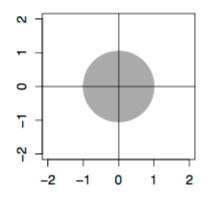
\includegraphics[width=.7525in]{stuffs/regularization_prior3_R.png} &
 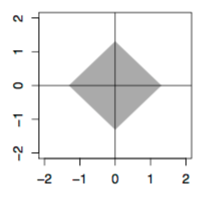
\includegraphics[width=.75in]{stuffs/regularization_prior3_L.png} &
  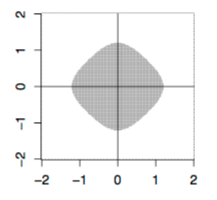
\includegraphics[width=.7525in]{stuffs/regularization_prior3_C.png} &
 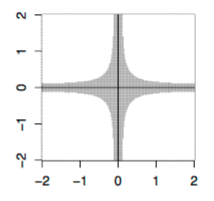
\includegraphics[width=.75in]{stuffs/regularization_prior3_H.png} \\
 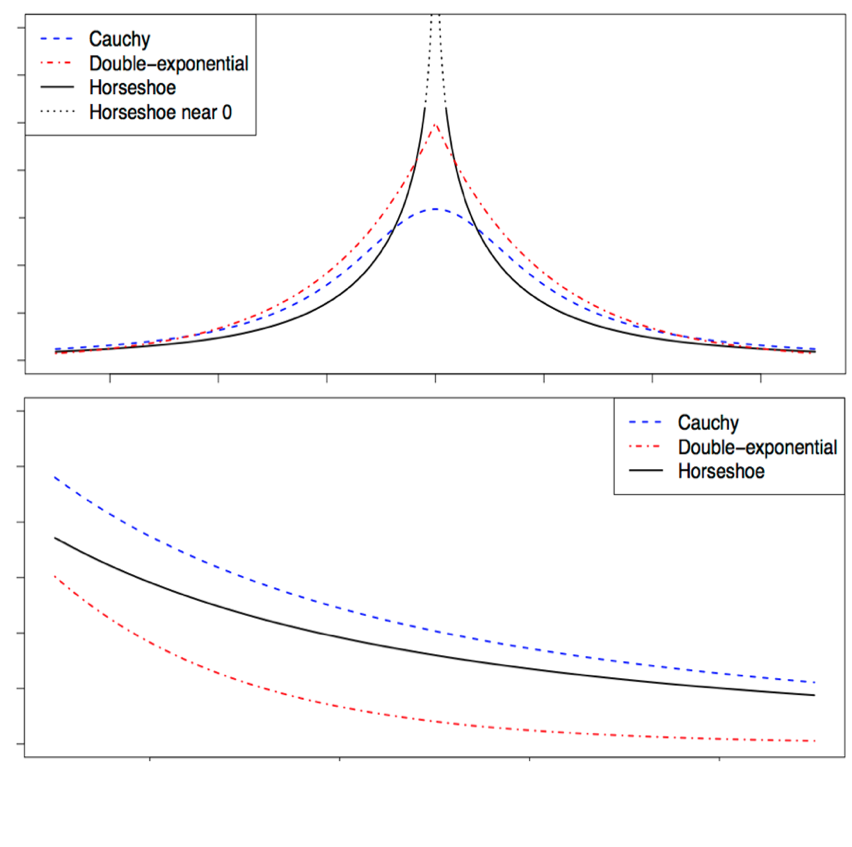
\includegraphics[width=.5525in]{stuffs/regularization_prior2.png}\textcolor{white}{\tiny ...}
 &
 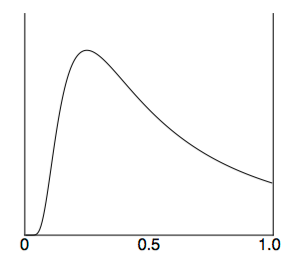
\includegraphics[width=.65in]{stuffs/regularization_prior4_L.png} &
  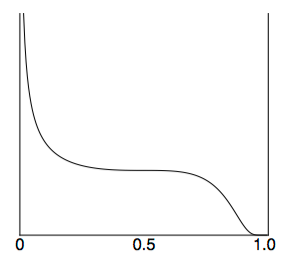
\includegraphics[width=.65in]{stuffs/regularization_prior4_C.png} &
 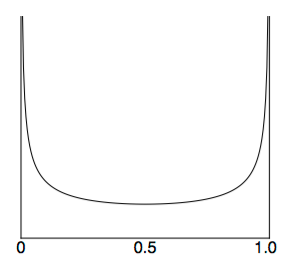
\includegraphics[width=.65in]{stuffs/regularization_prior4_H.png} \\
\multicolumn{1}{c}{\tiny$\quad$Tails}& \multicolumn{3}{c}{\tiny $\quad$Implied shrinkage prior profiles from none (0) to total (1) shrinkage}
  \end{tabular}
\end{figure}
}
}

\frame
{
 \frametitle{Objectives}
\begin{enumerate}
\item Understand generative versus predictive modeling
\item<2-> Understand ``covariance matrix difficulties'' when $q > n$
\item<3-> Understand how ``Naive Bayes'' comes to the rescue
\item<4-> Understand what Naive Bayes classification is \& how it works
\item<5-> Understand how Naive Bayes can be applied to NLP problems
\item<6-> Know that Naive Bayes is super undemanding computationally
\end{enumerate}

}


\frame
{
 \frametitle{Conditional versus joint models}
\begin{itemize}
\item Conditional/Predictive/Discriminative\\
\textcolor{gray}{(``outcome given features'')}
$$f(Y_i|{\boldsymbol x}_i)$$
\item<2-> Joint $\rightarrow$ Generative \textcolor{gray}{(``features given outcome'')}
$$f({\boldsymbol X}_i|Y_i) \rightarrow  f(Y_i,{\boldsymbol X}_i) \rightarrow f(Y_i|{\boldsymbol X}_i)$$
\item[]<2-> So we want to model ${\boldsymbol X}_i|Y_i$... in order to get ${Y_i|\boldsymbol X}_i$

\item[]
\item[]<3-> \textcolor{gray}{For categorical $Y_i \in \{k: k = 1,2, \cdots K \}$ 
\begin{align*}
f(Y_i,{\boldsymbol X}_i) = {}& \sum_{k=1}^K \Pr(Y_i=k) f({\boldsymbol X}_i|Y_i=k) \\
= {}& \sum_{k=1}^K \pi_k f_k({\boldsymbol X}_i) \\
\text{so what we need is } \Longrightarrow \textcolor{white}{\;=}{} & f({\boldsymbol X}_i|Y_i=k) \equiv f_k({\boldsymbol X}_i)
\end{align*}}
\end{itemize}
}


\frame
{
 \frametitle{Multivariate Normal (MVN) and Multinomial (MN)}

$$
\left[\begin{array}{cccc}
X_{11}&X_{12} & \cdots & X_{1q} \\
X_{21}&X_{22} & \cdots & X_{2q} \\
\vdots &\vdots &\ddots&\vdots \\\hline
X_{i1}&X_{i2} & \cdots & X_{iq} \\ \hline
\vdots &\vdots &\ddots&\vdots \\
X_{n1}&X_{n2} & \cdots & X_{nq} \\
\end{array}\right]
$$

\begin{align*}
{\boldsymbol X}_i ={} (X_{i1}, X_{i2}, \cdots, X_{iq})^T \sim & MVN({\boldsymbol \mu}_{q\times1},\Sigma_{q \times q}) \\
{}& (2\pi)^{-\frac{k}{2}} |\Sigma|^{-\frac{1}{2}} e^{-\frac{1}{2} ({\boldsymbol X_i} - {\boldsymbol \mu})^T \Sigma^{-1}({\boldsymbol X_i} - {\boldsymbol \mu})}\\
{}\\
{\boldsymbol X}_i ={} (X_{i1}, X_{i2}, \cdots, X_{iq})^T \sim & MN({\boldsymbol p}_{q\times1}, n_i)\\
{}& \frac{n_i!}{\prod_{j=1}^pX_{ij}!} \prod_{j=1}^q p_j^{X_{ij}}
\end{align*}




}



\frame
{
 \frametitle{Multivariate Models}
\begin{itemize}
\item 
${\boldsymbol X}_i \sim MVN({\boldsymbol \mu}_{q\times1},\Sigma_{q \times q})$ 
\item[] i.e.,
$${\boldsymbol X}_i \equiv  \left[\begin{array}{c} X_1 \\ X_2 \\ \vdots\\ X_q \end{array} \right] \sim MVN\left(
 \left[\begin{array}{c} \mu_{\textcolor{gray}{X_1}} \\ \mu_{\textcolor{gray}{X_2}} \\ \vdots\\ \mu_{\textcolor{gray}{X_q}} \end{array} \right]_,
\left[\begin{array}{cccc}\sigma^2_{\textcolor{gray}{X_1}}&\sigma_{\textcolor{gray}{X_1X_2}} & \cdots & \sigma_{\textcolor{gray}{X_1X_q}}\\ 
\sigma_{\textcolor{gray}{X_2X_1}} &\sigma^2_{\textcolor{gray}{X_2}}&  \cdots & \sigma_{\textcolor{gray}{X_2X_q}}\\
\vdots &\vdots&  \ddots & \vdots\\
\sigma_{\textcolor{gray}{X_qX_1}} & \sigma_{\textcolor{gray}{X_qX_2}} &   \cdots & \sigma^2_{\textcolor{gray}{X_q}}\\ \end{array}\right]\right)$$
\item<2-> What is $n$? And how do we estimate $\mu_{\textcolor{gray}{X_j}}, \sigma^2_{\textcolor{gray}{X_j}}, \sigma_{\textcolor{gray}{X_jX_{j'}}}?$
\end{itemize}
}

\frame
{
 \frametitle{Multivariate Models}
\begin{itemize}
\item 
${\boldsymbol X}_i   \sim MVN({\boldsymbol \mu}_{q\times1},\Sigma_{q \times q})$ 
\item[] i.e.,
$${\boldsymbol X}_i \equiv  \left[\begin{array}{c} X_1 \\ X_2 \\ \vdots\\ X_q \end{array} \right] \sim MVN\left(
 \left[\begin{array}{c} \mu_{\textcolor{gray}{X_1}} \\ \mu_{\textcolor{gray}{X_2}} \\ \vdots\\ \mu_{\textcolor{gray}{X_q}} \end{array} \right]_,
\left[\begin{array}{cccc}\sigma^2_{\textcolor{gray}{X_1}}&\;\;\;0\;\;\;& \cdots & \;\;\;\;0\;\;\;\\ 
0&\sigma^2_{\textcolor{gray}{X_2}}&  \cdots & 0\\
\vdots &\vdots&  \ddots & \vdots\\
\;\;\;\;0\;\;\; & 0 &   \cdots & \sigma^2_{\textcolor{gray}{X_q}}  \\ \end{array}\right]\right)$$
\item<1-> What does this matrix specify? And why use it? \textcolor{white}{$\sigma^2_{\textcolor{white}{X_j}}$}

\end{itemize}
}

\frame
{
 \frametitle{Multivariate Models}
 
 \vspace{.6em}
\begin{itemize}
\item 
${\boldsymbol X}_i   \sim MN({\boldsymbol p}_{q\times1}, n_i) \textcolor{white}{\Sigma_{q \times q}}$ 
\item[] i.e.,
$${\boldsymbol X}_i \equiv  \left[\begin{array}{c} X_1 \\ X_2 \\ \vdots\\ X_q \end{array} \right] \sim MN\left(
 \left[\begin{array}{c} p_{\textcolor{gray}{X_1}} \\ p_{\textcolor{gray}{X_2}} \\ \vdots\\ p_{\textcolor{gray}{X_q}} \end{array} \right]_, n_i \right) \textcolor{white}{\left[\begin{array}{cccc}\sigma^2_{\textcolor{white}{X_1}}&\;\;\;0\;\;\;& \cdots & \;\;\;\;0\;\;\;\\ 
0&\sigma^2_{\textcolor{white}{X_2}}&  \cdots & 0\\
\vdots &\vdots&  \ddots & \vdots\\
\;\;\;\;0\;\;\; & 0 &   \cdots & \sigma^2_{\textcolor{white}{X_q}}  \\ \end{array}\right]}$$
\item<1-> Multinomial model counts are (in)dependent? \textcolor{white}{$\sigma^2_{\textcolor{white}{X_j}}$}
\item<2-> What can we model with this? \onslide<3->{How 'bout text documents?}
\end{itemize}
}


\frame
{
 \frametitle{\emph{Multiple} Multivariate Models}
 
 \vspace{.6em}
\begin{itemize}
\item 
${\boldsymbol X}_i   \sim MN({\boldsymbol p}_{q\times1}, n_i) \textcolor{white}{\Sigma_{q \times q}}$ 
\item[] i.e.,
$${\boldsymbol X}_i \equiv  \left[\begin{array}{c} X_1 \\ X_2 \\ \vdots\\ X_q \end{array} \right] \sim MN\left(
 \left[\begin{array}{c} p_{k\textcolor{gray}{X_1}} \\ p_{k\textcolor{gray}{X_2}} \\ \vdots\\ p_{k\textcolor{gray}{X_q}} \end{array} \right]_, n_i \right) \textcolor{white}{\left[\begin{array}{cccc}\sigma^2_{\textcolor{white}{X_1}}&\;\;\;0\;\;\;& \cdots & \;\;\;\;0\;\;\;\\ 
0&\sigma^2_{\textcolor{white}{X_2}}&  \cdots & 0\\
\vdots &\vdots&  \ddots & \vdots\\
\;\;\;\;0\;\;\; & 0 &   \cdots & \sigma^2_{\textcolor{white}{X_q}}  \\ \end{array}\right]}$$
\item<1-> Multinomial model counts are (in)dependent? \textcolor{white}{$\sigma^2_{\textcolor{white}{X_j}}$}
\item<1-> What can we model with this? \onslide<1->{How 'bout text documents?}
\end{itemize}
}




\frame
{
 \frametitle{\emph{Multiple} Multivariate Models}
 
 
 \begin{columns}
 \begin{column}{.6\textwidth}
 \vspace{-1em}
$$ \displaystyle {\boldsymbol X}_i \equiv  \left[\begin{array}{c} X_1 \\ X_2 \\ \vdots\\ X_q \end{array} \right] \sim MN\left(
 \left[\begin{array}{c} p_{k\textcolor{gray}{X_1}} \\ p_{k\textcolor{gray}{X_2}} \\ \vdots\\ p_{k\textcolor{gray}{X_q}} \end{array} \right]_, n_i \right) \textcolor{white}{\left[\begin{array}{cccc}\sigma^2_{\textcolor{white}{X_1}}&\;\;\;0\;\;\;& \cdots & \;\;\;\;0\;\;\;\\ 
0&\sigma^2_{\textcolor{white}{X_2}}&  \cdots & 0\\
\vdots &\vdots&  \ddots & \vdots\\
\;\;\;\;0\;\;\; & 0 &   \cdots & \sigma^2_{\textcolor{white}{X_q}}  \\ \end{array}\right]}$$

\hspace{.2cm} 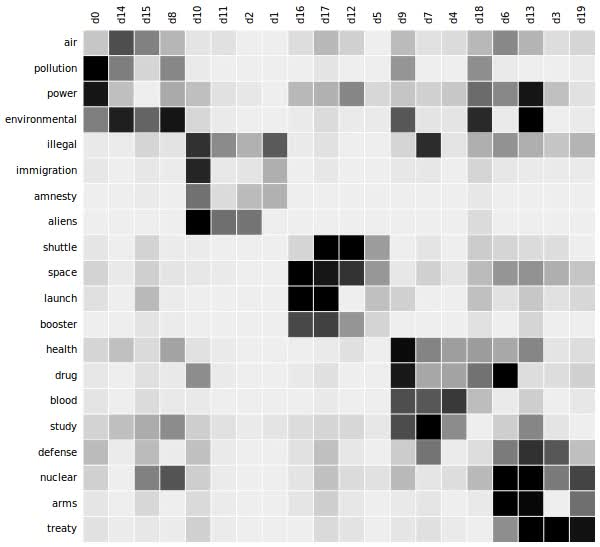
\includegraphics[width=2.225in, height=2.225in]{stuffs/Topic_model_scheme.jpg} 

\end{column}
 \begin{column}{.45\textwidth}
\vspace{-2.5em}
\footnotesize
\begin{itemize}

\item[]<2->

\begin{align*}
{}& f(Y_i,{\boldsymbol X}_i) \\
 = {}& \sum_{k=1}^K \Pr(Y_i=k) f({\boldsymbol X}_i|Y_i=k) \\
= {}& \sum_{k=1}^K \pi_k f_k({\boldsymbol X}_i) 
\end{align*}


\item[]<3-> $\pi_k \equiv \Pr(Y_i=k)$\\ estimated with 
$$\frac{1}{n}\sum 1_{[Y_i=k]}$$
\item[]
\item[]<4-> $f_k({\boldsymbol X}_i) \equiv f({\boldsymbol X}_i|Y_i=k)$\\ estimated with
$$ MN\left(\left[\begin{array}{c} X_1 \\ X_2 \\ \vdots\\ X_q \end{array} \right] \Bigg|
 \left[\begin{array}{c} \hat p_{k\textcolor{gray}{X_1}} \\ \hat p_{k\textcolor{gray}{X_2}} \\ \vdots\\ \hat p_{k\textcolor{gray}{X_q}} \end{array} \right]_, n_i \right) $$
\item[]
\end{itemize}

\end{column}
\end{columns}

}



\frame
{
 \frametitle{Why is this even called \emph{Bayes}? Why is this called \emph{Naive}?}
 
 
 \begin{columns}
 
  \begin{column}{.6\textwidth}
\vspace{-2.5em}
\begin{align*}
{} & \onslide<2->{\Pr(Y_i=k|  {\boldsymbol X}_i)}\\
\onslide<2->{= {}&\frac{f({\boldsymbol X}_i|Y_i=k)\Pr(Y=k)}{f({\boldsymbol X}_i)}}\\
\\
%\onslide<3->{= {}& \frac{f({\boldsymbol X}_i,Y_i=k)}{f({\boldsymbol X}_i)}} \\
\onslide<3->{= {}& \frac{\pi_{k} f_{k}({\boldsymbol X}_i)}{\sum_{k'=1}^K \pi_{k'} f_{k'}({\boldsymbol X}_i)}}\\
\onslide<4->{\propto {}& \pi_{k} f_{k}({\boldsymbol X}_i)}\\
\onslide<5->{\propto {}& \pi_{k} \hat p_{k\textcolor{gray}{X_1}}^{X_{i1}} \cdot \hat p_{k\textcolor{gray}{X_2}}^{X_{i2}}  \cdots \hat p_{k\textcolor{gray}{X_q}}^{X_{ip}}}\\
\onslide<6->{= {}& \pi_{k} \prod_{\underline{word} \in  words} \hat p_{k \underline{word}}}\\
\onslide<7->{{}& \text{Notice how probability of a word}}\\
\onslide<7->{{}& \text{is independent of previous words}}\\
\onslide<8->{\not = {}& \pi_{k} \prod_{\underline{word} \in  words} \hat p_{k \underline{word|\text{previous words}}}}
\end{align*}

\end{column}


 \begin{column}{.45\textwidth}
\vspace{-2.5em}
\footnotesize
\begin{itemize}

\item[]<1->

\begin{align*}
{}& f(Y_i,{\boldsymbol X}_i) \\
 = {}& \sum_{k=1}^K \Pr(Y_i=k) f({\boldsymbol X}_i|Y_i=k) \\
= {}& \sum_{k=1}^K \pi_k f_k({\boldsymbol X}_i) 
\end{align*}


\item[]<1-> $\pi_k \equiv \Pr(Y_i=k)$\\ estimated with 
$$\frac{1}{n}\sum 1_{[Y_i=k]}$$
\item[]
\item[]<1-> $f_k({\boldsymbol X}_i) \equiv f({\boldsymbol X}_i|Y_i=k)$\\ estimated with
$$ MN\left(\left[\begin{array}{c} X_1 \\ X_2 \\ \vdots\\ X_q \end{array} \right] \Bigg|
 \left[\begin{array}{c} \hat p_{k\textcolor{gray}{X_1}} \\ \hat p_{k\textcolor{gray}{X_2}} \\ \vdots\\ \hat p_{k\textcolor{gray}{X_q}} \end{array} \right]_, n_i \right) $$
\item[]
\end{itemize}

\end{column}


\end{columns}

}



\frame
{
 \frametitle{Tricks}
 
 Laplace Smoothing: 
$$\hat p_{k\textcolor{gray}{X_j}} = \frac{\# (\text{times $X_j$ appears in Class }k)+ \alpha}{\# (\text{words in Class }k) + \alpha \times |\text{Vocab}|}$$\\${}$\\


Exponentiating the sum of log probabilities: 
\begin{align*}
{} & \Pr(Y_i=k|  {\boldsymbol X}_i)\\
= {} & \frac{\pi_{k} \hat p_{k\textcolor{gray}{X_1}}^{X_{i1}} \cdot \hat p_{k\textcolor{gray}{X_2}}^{X_{i2}}  \cdots \hat p_{k\textcolor{gray}{X_q}}^{X_{ip}}}{\sum_{k'=1}^K\pi_{k'} \hat p_{k'\textcolor{gray}{X_1}}^{X_{i1}} \cdot \hat p_{k'\textcolor{gray}{X_2}}^{X_{i2}}  \cdots \hat p_{k'\textcolor{gray}{X_q}}^{X_{ip}}}
= 
\frac{1}{\sum_{k'=1}^K
\frac{
\pi_{k'} \hat p_{k'\textcolor{gray}{X_1}}^{X_{i1}} \cdot \hat p_{k'\textcolor{gray}{X_2}}^{X_{i2}}  \cdots \hat p_{k'\textcolor{gray}{X_q}}^{X_{ip}}}{\pi_{k} \hat p_{k\textcolor{gray}{X_1}}^{X_{i1}} \cdot \hat p_{k\textcolor{gray}{X_2}}^{X_{i2}}  \cdots \hat p_{k\textcolor{gray}{X_q}}^{X_{ip}}
}}\\
= {} &
\frac{1}{\sum_{k'=1}^K \frac{\pi_{k'}}{\pi_{k}}
exp\left( \sum_{j=1}^q log( \hat p_{k'\textcolor{gray}{X_j}}^{X_{ij}})
-
\sum_{j=1}^q log( \hat p_{k\textcolor{gray}{X_j}}^{X_{ij}})
 \right) }\\
\end{align*}

}



\frame
{
 \frametitle{What is the assumption on the covariance matrix doing?}

Back to the MVN... 
\vspace{-1em}
\begin{columns}
\begin{column}{.36\textwidth}

\begin{align*}
{}& \Pr(Y_i=k|  {\boldsymbol X}_i)\\
 \propto {}& \pi_{k} f_{k}({\boldsymbol X}_i)\\
 = {}& \pi_{k}\prod_{j=1}^q f_k(X_{ji})
\end{align*} 

\end{column}
\begin{column}{.5\textwidth}


$$ \left[\begin{array}{cccc}\hat \sigma^2_{k\textcolor{gray}{X_1}}&\;\;\;0\;\;\;& \cdots & \;\;\;\;0\;\;\;\\ 
0&\hat \sigma^2_{k\textcolor{gray}{X_2}}&  \cdots & 0\\
\vdots &\vdots&  \ddots & \vdots\\
\;\;\;\;0\;\;\; & 0 &   \cdots & \hat \sigma^2_{k\textcolor{gray}{X_q}}  \\ \end{array}\right] $$

\end{column}
\end{columns}


\begin{figure}
\centering
 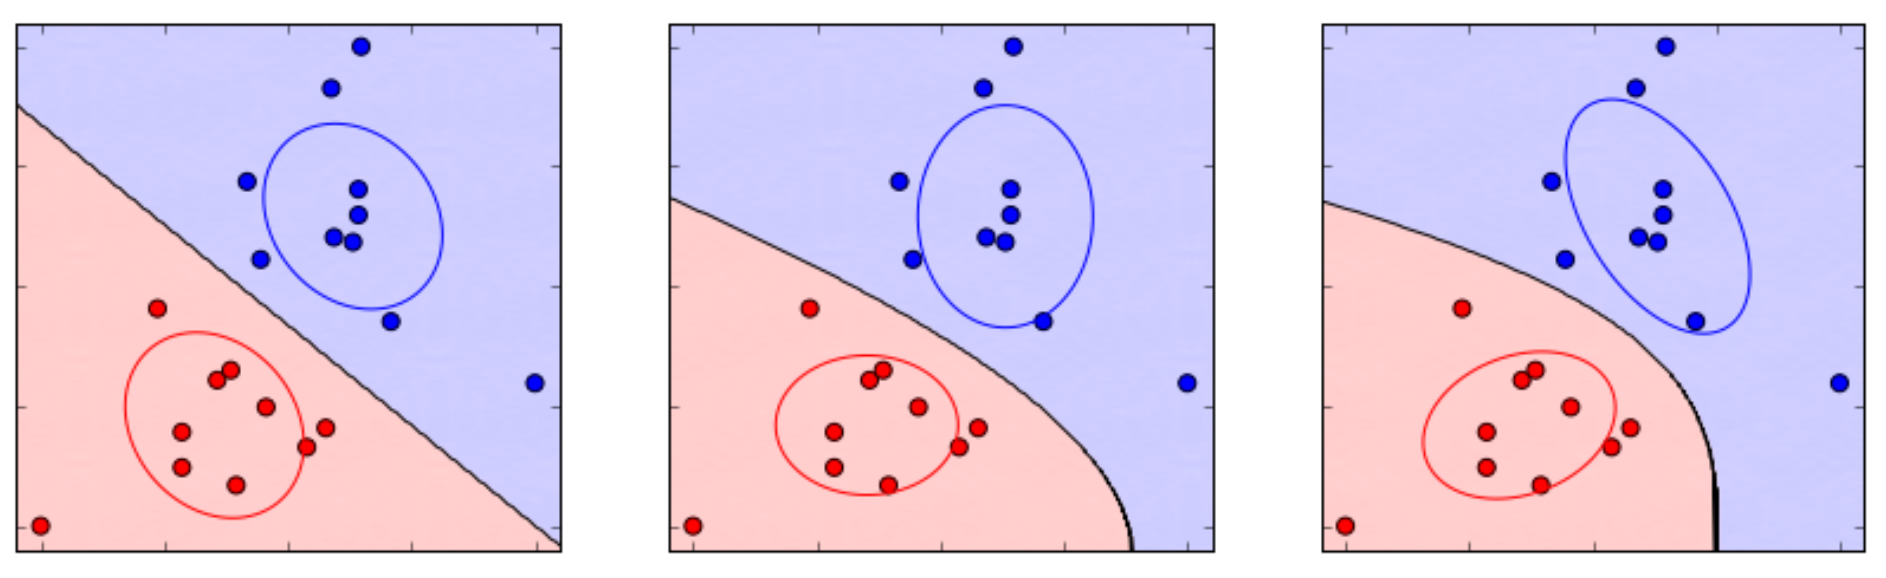
\includegraphics[width=4in]{stuffs/linear_discriminants.png}
 
\tiny
\onslide<2->{\hspace{.5em} Linear Discriminant Analysis (LDA)  \hspace{5em} Naive Bayes \hspace{4.25em} Quadratic Discriminant Analysis (QDA)}

\onslide<3->{\Huge \textcolor{red}{$\Uparrow\Uparrow\Uparrow\Uparrow\Uparrow$}}
 

\end{figure}
}


\frame
{
 \frametitle{Parting comments}

\begin{itemize}
\item Truly correlated features can hamper Naive Bayes (NB)
\item<2-> Probability estimates are unreliable with the naive assumption
\item<3-> But NB classifications can be workable... but
\item<4-> NB is typically outperformed by less naive methodologies
\item<5->[] However...
\item<6-> NB is super undemanding computationally:
\item<7->[] NB can handle huge data sets very quickly -- i.e., in real time
\item<8->[] NB can handle wide data sets other methodologies can't... 
\item<9-> And NB is very simple to implement and use...
\item<10->[]  \textcolor{gray}{Although isn't \emph{everything} in scikit-learn?}
\end{itemize}

}


\end{document}





\frame
{
 \frametitle{Covariance Matrices}
\begin{itemize}
\item 
${\boldsymbol X}_i \sim MVN({\boldsymbol \mu}_q,\Sigma_{q \times q})$ 
\item[] i.e.,
$${\boldsymbol X}_i \equiv  \left[\begin{array}{c} X_1 \\ X_2 \\ \vdots\\ X_q \end{array} \right] \sim MVN\left(
 \left[\begin{array}{c} \mu_{\textcolor{gray}{X_1}} \\ \mu_{\textcolor{gray}{X_2}} \\ \vdots\\ \mu_{\textcolor{gray}{X_q}} \end{array} \right]_,
\left[\begin{array}{cccc}\sigma^2_{\textcolor{gray}{X_1}}&\sigma_{\textcolor{gray}{X_1X_2}} & \cdots & \sigma_{\textcolor{gray}{X_1X_q}}\\ 
\sigma_{\textcolor{gray}{X_2X_1}} &\sigma^2_{\textcolor{gray}{X_2}}&  \cdots & \sigma_{\textcolor{gray}{X_2X_q}}\\
\vdots &\vdots&  \ddots & \vdots\\
\sigma_{\textcolor{gray}{X_qX_1}} & \sigma_{\textcolor{gray}{X_qX_2}} &   \cdots & \sigma^2_{\textcolor{gray}{X_q}}\\ \end{array}\right]\right)$$
\item<2-> $\hat \Sigma_{q\times p} = \frac{\sum_{i=1}^{n}({\boldsymbol X}_i - \bar {\boldsymbol X})_{q\times 1}({\boldsymbol X}_i - \bar {\boldsymbol X})^T_{q\times 1}}{n-1}$
\item<3-> If $n < p$, the \emph{rank} of $\hat \Sigma_{q\times p}$ is $n$ \\
\textcolor{gray}{since it is a linear combination of only with $n$ \emph{independent} ${\boldsymbol X}_i's$}
\item<4-> Thus, $\hat \Sigma_{q\times p}$ \emph{will not} be invertible
\item<5-> This is bad news since the pdf of ${\boldsymbol X} \sim MVN({\boldsymbol \mu}, \Sigma)$ is 

$$(2\pi)^{-\frac{k}{2}} |\Sigma|^{-\frac{1}{2}} e^{-\frac{1}{2} ({\boldsymbol X} - {\boldsymbol \mu})^T \Sigma^{-1}({\boldsymbol X} - {\boldsymbol \mu})}$$

\end{itemize}
}


\frame
{
 \frametitle{Covariance Matrices}
\begin{itemize}
\item 
${\boldsymbol X}_i   \sim MVN({\boldsymbol \mu}_q,\Sigma_{q \times q})$ 
\item[] i.e.,
$${\boldsymbol X}_i \equiv  \left[\begin{array}{c} X_1 \\ X_2 \\ \vdots\\ X_q \end{array} \right] \sim MVN\left(
 \left[\begin{array}{c} \mu_{\textcolor{gray}{X_1}} \\ \mu_{\textcolor{gray}{X_2}} \\ \vdots\\ \mu_{\textcolor{gray}{X_q}} \end{array} \right]_,
\left[\begin{array}{cccc}\sigma^2_{\textcolor{gray}{X_1}}&\;\;\;0\;\;\;& \cdots & \;\;\;\;0\;\;\;\\ 
0&\sigma^2_{\textcolor{gray}{X_2}}&  \cdots & 0\\
\vdots &\vdots&  \ddots & \vdots\\
\;\;\;\;0\;\;\; & 0 &   \cdots & \sigma^2_{\textcolor{gray}{X_q}}  \\ \end{array}\right]\right)$$
\item $\hat \Sigma_{q\times p} = \frac{\sum_{i=1}^{n}({\boldsymbol X}_i - \bar {\boldsymbol X})_{q\times 1}({\boldsymbol X}_i - \bar {\boldsymbol X})^T_{q\times 1}}{n-1}$
\item If $n < p$, the \emph{rank} of $\hat \Sigma_{q\times p}$ is $n$ \\
\textcolor{gray}{since it is a linear combination of only with $n$ \emph{independent} ${\boldsymbol X}_i's$}
\item Thus, $\hat \Sigma_{q\times p}$ \emph{will not} be invertible
\item This is bad news since the pdf of ${\boldsymbol X} \sim MVN({\boldsymbol \mu}, \Sigma)$ is 

$$(2\pi)^{-\frac{k}{2}} |\Sigma|^{-\frac{1}{2}} e^{-\frac{1}{2} ({\boldsymbol X} - {\boldsymbol \mu})^T \Sigma^{-1}({\boldsymbol X} - {\boldsymbol \mu})}$$

\end{itemize}
}


\frame
{
 \frametitle{Covariance Matrices}
\begin{itemize}
\item 
${\boldsymbol X}_i  \sim MVN({\boldsymbol \mu}_q,\Sigma_{q \times q})$ 
\item[] i.e.,
$${\boldsymbol X}_i \equiv  \left[\begin{array}{c} X_1 \\ X_2 \\ \vdots\\ X_q \end{array} \right] \sim MVN\left(
 \left[\begin{array}{c} \mu_{\textcolor{gray}{X_1}} \\ \mu_{\textcolor{gray}{X_2}} \\ \vdots\\ \mu_{\textcolor{gray}{X_q}} \end{array} \right]_,
\left[\begin{array}{cccc}\sigma^2_{\textcolor{gray}{X_1}}&\;\;\;0\;\;\;& \cdots & \;\;\;\;0\;\;\;\\ 
0&\sigma^2_{\textcolor{gray}{X_2}}&  \cdots & 0\\
\vdots &\vdots&  \ddots & \vdots\\
\;\;\;\;0\;\;\; & 0 &   \cdots & \sigma^2_{\textcolor{gray}{X_q}} \\ \end{array}\right]\right)$$
\item \textcolor{white}{$\hat \Sigma_{q\times p} = \frac{\sum_{i=1}^{n}({\boldsymbol X}_i - \bar {\boldsymbol X})_{q\times 1}({\boldsymbol X}_i - \bar {\boldsymbol X})^T_{q\times 1}}{n-1}$} 
\hspace{-2.14in} $\sigma_{X_j}^2 = \frac{\sum_{i=1}^n (X_{ji} - \mu_{j})^2}{n-1} \text{ and } \sigma_{X_jX_k} = 0 \text{ for } j \not = k$
\item If $n < p$, the \emph{rank} of $\hat \Sigma_{q\times p}$ is $n$ \\
\textcolor{gray}{since it is a linear combination of only with $n$ \emph{independent} ${\boldsymbol X}_i's$}
\item Thus, $\hat \Sigma_{q\times p}$ \emph{will not} be invertible
\item This is bad news since the pdf of ${\boldsymbol X} \sim MVN({\boldsymbol \mu}, \Sigma)$ is 

$$(2\pi)^{-\frac{k}{2}} |\Sigma|^{-\frac{1}{2}} e^{-\frac{1}{2} ({\boldsymbol X} - {\boldsymbol \mu})^T \Sigma^{-1}({\boldsymbol X} - {\boldsymbol \mu})}$$

\end{itemize}
}


\frame
{
 \frametitle{Covariance Matrices}
\begin{itemize}
\item 
${\boldsymbol X}_i  \sim MVN({\boldsymbol \mu}_q,\Sigma_{q \times q})$ 
\item[] i.e.,
$${\boldsymbol X}_i \equiv  \left[\begin{array}{c} X_1 \\ X_2 \\ \vdots\\ X_q \end{array} \right] \sim MVN\left(
 \left[\begin{array}{c} \mu_{\textcolor{gray}{X_1}} \\ \mu_{\textcolor{gray}{X_2}} \\ \vdots\\ \mu_{\textcolor{gray}{X_q}} \end{array} \right]_,
\left[\begin{array}{cccc}\sigma^2_{\textcolor{gray}{X_1}}&\;\;\;0\;\;\;& \cdots & \;\;\;\;0\;\;\;\\ 
0&\sigma^2_{\textcolor{gray}{X_2}}&  \cdots & 0\\
\vdots &\vdots&  \ddots & \vdots\\
\;\;\;\;0\;\;\; & 0 &   \cdots & \sigma^2_{\textcolor{gray}{X_q}}  \\ \end{array}\right]\right)$$
\item \textcolor{white}{$\hat \Sigma_{q\times p} = \frac{\sum_{i=1}^{n}({\boldsymbol X}_i - \bar {\boldsymbol X})_{q\times 1}({\boldsymbol X}_i - \bar {\boldsymbol X})^T_{q\times 1}}{n-1}$} 
\hspace{-2.14in} $\sigma_{X_j}^2 = \frac{\sum_{i=1}^n (X_{ji} - \mu_{j})^2}{n-1} \text{ and } \sigma_{X_jX_k} = 0 \text{ for } j \not = k$
\item If $n < p$, the \emph{rank} of $\hat \Sigma_{q\times p}$ is $n$  \hspace{-1.31em} ${\boldsymbol\equiv} \;p$ \\
\textcolor{white}{since it was constructed with $n$ \emph{independent} $X_i's$}\hspace{-3.125in} \textcolor{gray}{because it's a $p\times p$ invertible diagonal matrix}
\item Thus, $\hat \Sigma_{q\times p}$ \emph{will not} be invertible
\item This is bad news since the pdf of ${\boldsymbol X} \sim MVN({\boldsymbol \mu}, \Sigma)$ is 

$$(2\pi)^{-\frac{k}{2}} |\Sigma|^{-\frac{1}{2}} e^{-\frac{1}{2} ({\boldsymbol X} - {\boldsymbol \mu})^T \Sigma^{-1}({\boldsymbol X} - {\boldsymbol \mu})}$$

\end{itemize}
}

\frame
{
 \frametitle{Covariance Matrices}
\begin{itemize}
\item 
${\boldsymbol X}_i  \sim MVN({\boldsymbol \mu}_q,\Sigma_{q \times q})$ 
\item[] i.e.,
$${\boldsymbol X}_i \equiv  \left[\begin{array}{c} X_1 \\ X_2 \\ \vdots\\ X_q \end{array} \right] \sim MVN\left(
 \left[\begin{array}{c} \mu_{\textcolor{gray}{X_1}} \\ \mu_{\textcolor{gray}{X_2}} \\ \vdots\\ \mu_{\textcolor{gray}{X_q}} \end{array} \right]_,
\left[\begin{array}{cccc}\sigma^2_{\textcolor{gray}{X_1}}&\;\;\;0\;\;\;& \cdots & \;\;\;\;0\;\;\;\\ 
0&\sigma^2_{\textcolor{gray}{X_2}}&  \cdots & 0\\
\vdots &\vdots&  \ddots & \vdots\\
\;\;\;\;0\;\;\; & 0 &   \cdots & \sigma^2_{\textcolor{gray}{X_q}}  \\ \end{array}\right]\right)$$
\item \textcolor{white}{$\hat \Sigma_{q\times p} = \frac{\sum_{i=1}^{n}({\boldsymbol X}_i - \bar {\boldsymbol X})_{q\times 1}({\boldsymbol X}_i - \bar {\boldsymbol X})^T_{q\times 1}}{n-1}$} 
\hspace{-2.14in} $\sigma_{X_j}^2 = \frac{\sum_{i=1}^n (X_{ji} - \mu_{j})^2}{n-1} \text{ and } \sigma_{X_jX_k} = 0 \text{ for } j \not = k$
\item If $n < p$, the \emph{rank} of $\hat \Sigma_{q\times p}$ is $n$  \hspace{-1.31em} ${\boldsymbol\equiv} \;p$ \\
\textcolor{white}{since it was constructed with $n$ \emph{independent} $X_i's$}\hspace{-3.125in} \textcolor{gray}{because it's a $p\times p$ invertible diagonal matrix}
\item Thus, $\hat \Sigma_{q\times p}$ \emph{will \textcolor{white}{not}} \textcolor{white}{be invertible} \hspace{-.9in}  \textbf{be invertible} 
\item This is bad news since the pdf of ${\boldsymbol X} \sim MVN({\boldsymbol \mu}, \Sigma)$ is 

$$(2\pi)^{-\frac{k}{2}} |\Sigma|^{-\frac{1}{2}} e^{-\frac{1}{2} ({\boldsymbol X} - {\boldsymbol \mu})^T \Sigma^{-1}({\boldsymbol X} - {\boldsymbol \mu})}$$

\end{itemize}
}

\frame
{
 \frametitle{Covariance Matrices}
\begin{itemize}
\item 
${\boldsymbol X}_i  \sim MVN({\boldsymbol \mu}_q,\Sigma_{q \times q})$ 
\item[] i.e.,
$${\boldsymbol X}_i \equiv  \left[\begin{array}{c} X_1 \\ X_2 \\ \vdots\\ X_q \end{array} \right] \sim MVN\left(
 \left[\begin{array}{c} \mu_{\textcolor{gray}{X_1}} \\ \mu_{\textcolor{gray}{X_2}} \\ \vdots\\ \mu_{\textcolor{gray}{X_q}} \end{array} \right]_,
\left[\begin{array}{cccc}\sigma^2_{\textcolor{gray}{X_1}}&\;\;\;0\;\;\;& \cdots & \;\;\;\;0\;\;\;\\ 
0&\sigma^2_{\textcolor{gray}{X_2}}&  \cdots & 0\\
\vdots &\vdots&  \ddots & \vdots\\
\;\;\;\;0\;\;\; & 0 &   \cdots & \sigma^2_{\textcolor{gray}{X_q}}  \\ \end{array}\right]\right)$$
\item \textcolor{white}{$\hat \Sigma_{q\times p} = \frac{\sum_{i=1}^{n}({\boldsymbol X}_i - \bar {\boldsymbol X})_{q\times 1}({\boldsymbol X}_i - \bar {\boldsymbol X})^T_{q\times 1}}{n-1}$} 
\hspace{-2.14in} $\sigma_{X_j}^2 = \frac{\sum_{i=1}^n (X_{ji} - \mu_{j})^2}{n-1} \text{ and } \sigma_{X_jX_k} = 0 \text{ for } j \not = k$
\item If $n < p$, the \emph{rank} of $\hat \Sigma_{q\times p}$ is $n$  \hspace{-1.31em} ${\boldsymbol\equiv} \;p$ \\
\textcolor{white}{since it was constructed with $n$ \emph{independent} $X_i's$}\hspace{-3.125in} \textcolor{gray}{because it's a $p\times p$ invertible diagonal matrix}
\item Thus, $\hat \Sigma_{q\times p}$ \emph{will \textcolor{white}{not}} \textcolor{white}{be invertible} \hspace{-.9in}  \textbf{be invertible} 
\item This is \textcolor{white}{bad} news since the pdf of ${\boldsymbol X} \sim MVN({\boldsymbol \mu}, \Sigma)$ is \hspace{-2.965in}{\footnotesize \underline{\textcolor{red}{good}}}

$$(2\pi)^{-\frac{k}{2}} |\Sigma|^{-\frac{1}{2}} e^{-\frac{1}{2} ({\boldsymbol X} - {\boldsymbol \mu})^T \Sigma^{-1}({\boldsymbol X} - {\boldsymbol \mu})}$$

\end{itemize}
}


\frame
{
 \frametitle{Time for some explicit clarification of the notation}

\begin{itemize}
\item[] Because there's a lot going on here and it \emph{is confusing...}
\item[]
\item<2->[] \underline{You need to be \emph{very careful} to keep everything straight} 
\item[]
\item<3-> ${\boldsymbol X}_i$ is a vector $p$ of features related to outcome $Y_i$
\item[]
\item<4-> Each of the $p$ features in ${\boldsymbol X}_i$ is referred to as $X_j$
\item[]
\item<5-> A specific value for feature $X_j$ of outcome $Y_i$ is notated as $X_{ji}$
\item[]
\item<6-> Outcome $Y_i \in \{k: k = 1,2, \cdots K \}$ is categorial,  
taking on one of $K$ possible outcome values referred to as $k$
\end{itemize}

}


\frame
{
 \frametitle{Estimating the joint distribution of features and outcomes}

$$f(Y_i,{\boldsymbol X}_i) = \sum_{k=1}^K \pi_k f_k({\boldsymbol X}_i)$$


\begin{itemize}
\item<2-> Estimate $\pi_k \equiv \Pr(Y_i=k)$ with $\frac{1}{n}\sum 1_{[Y_i=k]}$
\item<3-> Estimate $f_k({\boldsymbol X}_i) \equiv f({\boldsymbol X}_i|Y_i=k)$ with


$${\boldsymbol X}_i \sim MVN\left(
 \left[\begin{array}{c} \hat \mu_{k\textcolor{gray}{X_1}} \\ \hat \mu_{k\textcolor{gray}{X_2}} \\ \vdots\\ \mu_{k\textcolor{gray}{X_q}} \end{array} \right]_,
\left[\begin{array}{cccc}\hat \sigma^2_{k\textcolor{gray}{X_1}}&\;\;\;0\;\;\;& \cdots & \;\;\;\;0\;\;\;\\ 
0&\hat \sigma^2_{k\textcolor{gray}{X_2}}&  \cdots & 0\\
\vdots &\vdots&  \ddots & \vdots\\
\;\;\;\;0\;\;\; & 0 &   \cdots & \hat \sigma^2_{k\textcolor{gray}{X_q}}  \\ \end{array}\right]\right)$$

where 
$ \hat \sigma_{k\textcolor{gray}{X_j}}^2 = \frac{\overset{n}{\underset{i=1: Y_i=k}{\sum}} (X_{ji} - \bar X_{j})^2}{\left(\overset{n}{\underset{i=1: Y_i=k}{\sum}} 1\right)-1}$
and
$ \hat \mu_{k\textcolor{gray}{X_j}} = \frac{\overset{n}{\underset{i=1: Y_i=k}{\sum}} X_{ji}}{\overset{n}{\underset{i=1: Y_i=k}{\sum}} 1}$

\end{itemize}
}




\frame
{
 \frametitle{Why is this even called Bayes?}

\begin{columns}
\begin{column}{.4\textwidth}

\end{column}
\begin{column}{.6\textwidth}
\begin{figure}
\centering
\onslide<5->{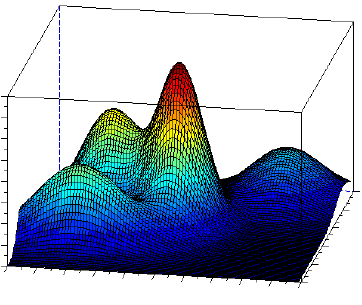
\includegraphics[width=2.4in]{stuffs/mixture.png}}
\end{figure}
\end{column}
\end{columns}

\onslide<6->{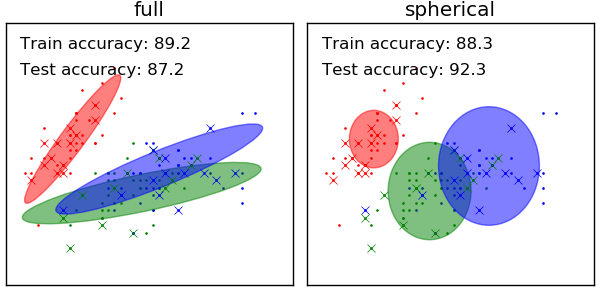
\includegraphics[width=2.15in]{stuffs/mix2.png}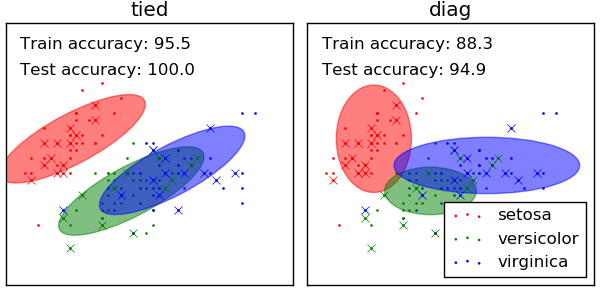
\includegraphics[width=2.15in]{stuffs/mix2b.png}}
}


\frame
{
 \frametitle{Multinomial Models for Word Counts in Text}


 
}




\frame
{
 \frametitle{Other models for feature $X_j$ }


\begin{itemize}
\item So far we've assumed that feature $X_j$ is 
\begin{itemize}
\item[(a)]<2-> continuous valued and \emph{normally distributed} 
\item[(b)]<3-> independent of the other features $X_{j'}$ for $j' \not = j$
\end{itemize}
\item<4->[] I.e., we said ${\boldsymbol X}_i$ is $MVN$ with a diagonal covariance matrix
\item<5-> But we can also have features $X_j$ that are  
\item<6->[] Multinomial for categorical $X_j$ \textcolor{red}{(e.g., counts of words in doc)}
\item<7->[] Bernoulli for indicator $X_j$ \textcolor{red}{(e.g., appearance of word in doc)}\\
\textcolor{pink}{\emph{both of these assume features (e.g., words) are independent}}\\
\item<8->[] \textcolor{gray}{And so on... depending on our choices for modeling $X_j$}
\item<9-> Can we use different types of $X_j$ at the same time? \onslide<9->{\textcolor{gray}{Of course}}
\item[]<10-> $$f_k({\boldsymbol X}_i) = \prod_{j=1}^q f_k(X_{ji})$$
\item[]<11-> As long as we assume the features are independent...
\item[]<12-> \textcolor{gray}{That's actually exactly what we did with the diagonal $MVN:$} \onslide<13->{\textcolor{gray}{assumed $X_j$'s independent normals}} \onslide<13->{\textcolor{gray}{\& multiplied $\Longrightarrow MVN$}}
\end{itemize}

}

\frame
{
 \frametitle{And don't forget...}


$$\text{multiply, multiply, multiply -- it's that easy}$$

\begin{itemize}
\item<2-> E.g., in classifying news story types

$$\hat \pi_{k} = \frac{\text{number of sports articles}}{\text{total number of articles}}$$

\vspace{.5em}
\onslide<3->{$\;\;f_{\text{sports}}(\text{``Cleveland's 52-year championship drought}$ \\$\quad\quad\quad\quad\text{ended with the 2015/16 NBA season...''})$}\\${}$
\vspace{-.25em}
\footnotesize
\onslide<4->{$\text{$=$}\Pr(\text{``Cleveland's"}|\text{sports})\Pr(\text{``52-year"}|\text{sports})\Pr(\text{``Championship"}|\text{sports})\cdots$}\\${}$\\
\vspace{.25em}
\normalsize
\onslide<5->{$\text{$=$}\frac{\text{\# ``Cleveland's" in sports + $\alpha$}}{\text{\# words in sports + $\alpha \times$ total \# words}}\text{$\cdot$}\frac{\text{\# ``52-year" in sports + $\alpha$}}{\text{\# words in sports + $\alpha \times$ total \# words}} {\footnotesize \cdots}$}

\item[]
\item<6-> \textcolor{gray}{The $\alpha$ is \emph{Laplace smoothing} -- it avoids multiplying by 0}
\item<7-> \textcolor{gray}{You'll probably also want to take a $log$...}

\end{itemize}


}


